\section{Background}
\label{sec:background}

%\fixmedp{maybe introduce the term prefix check here too?}

This section first reviews the Unix directory semantics which a directory cache must support;
and then explains how directory caches are implemented in  modern OSes, 
including Linux, FreeBSD, Solaris, Mac OS X, and Windows.

%\fixmedp{Please cite the relevant books or other sources you got this info from}

\subsection{Unix Directory Hierarchy Semantics}

%% In a hierarchical file system, as Unix variants provide, 
%% a user must be able to search all parent directories to access a given file.
%% In the case of traditional Unix permissions specifically, this means that

The most common operation a directory cache performs is a {\bf lookup},
which maps a path string onto an in-memory inode structure.
Lookup is called by all path-based system calls, including {\tt open}, {\tt stat}, and {\tt unlink}.
Lookup includes a check that the user has appropriate search permission from 
the process's root or current working directory to the file,
which we call a {\bf prefix check}.

For instance, 
in order for Alice to read {\tt /home/alice/\fnone{}}, she must have search permission 
on directories {\tt /}, {\tt /home}, and {\tt /home/alice}, as well as read
permission on file {\tt \fnone{}}.  In the interest of frugality, 
the execute permission bit on directories encodes search permission.
Search is distinct from read permission in that search only allows a user to query whether 
a file exists, but not enumerate the contents (except by brute force)~\citep{ritchie74unix}.
% querying of all possible file names)
SELinux~\citep{selinux} and other security-hardened Linux variants~\citep{wright+lsm, apparmor},
may determine search permission based on a number of factors beyond the execute bit, such as a process's role, or the extended attributes of a directory.


%% Several system calls, such as {\tt open}, {\tt stat}, and {\tt link}, 
%% must map a path string onto an in-memory inode structure, checking 
%% search permissions of each enclosing directory from the process's root or current working directory.
%% We call this kernel-internal mapping operation a {\bf lookup}.

%% Because a lookup must check hierarchical permissions, lookup implementations
%% traverse the directory hierarchy both to find the relevant inode and to check search permissions.
%% One contribution of this paper is to demonstrate how lookup performance can be improved substantially
%% by decoupling search permission checks from finding the inode mapped by a path (\S\ref{sec:dcache}).
%% Moreover, this paper shows how to efficiently cache search permissions, which change very infrequently on most systems,
%% avoiding this hierarchical traversal on the hit path in the common case.

%% The techniques for search permission caching in this paper are general.
%% SELinux~\citep{selinux} or other security-hardened Linux variants~\citep{wright+lsm, apparmor},
%% may determine search permission based on a number of factors beyond the execute bit, such as a process's role, or the extended attributes of a directory.
%% \S\ref{sec:dcache:selinux} shows that our permission caching techniques generalize to these platforms
%% because they do not depend on {\em how} the access checks are implemented, only that
%% the inputs can be identified and that the check itself is deterministic on these inputs.


%% \fixmedp{I think we can assume people understand that files are organized in a tree structure, and know ., .., etc.  I would very briefly talk about hierarchical permissions, mapping path strings to an inode/vnode in memory, and then just remind people more formally what the rules are (all directories you traverse must have X bit set for you), and how this gets a little more complicated with SELinux or other models.  }

%% The design of most Unix file systems are closely related
%% with their {\bf hierarchical structures}.

%% Almost all Unix operating systems structure their file system layers
%% as {\bf trees of objects}.
%% A Unix-compatible file system contains three types of objects:
%% containers ({\bf directories}), regular objects ({\bf files})
%% and special objects ({\bf links}, {\bf devices} and {\bf mount points}).
%% In a tree of file system, regular objects and special objects
%% are always leaves,
%% and only containers can be internal nodes that have one or more children.
%% Links and mount points can reference to other containers or objects,
%% thus creating cross-edges in the tree. 

%% Unix file system often describes objects by {\bf paths of tree traversal}.
%% The descriptor for an object
%% consists of identifiers matched with named edges to cross to reach the target object.
%% For example, a path like {\tt /a/b/c} will start at the root of tree,
%% and reach the target object by crossing the edges
%% named {\tt a}, {\tt b} and {\tt c} respectively.
%% When the walk passes by a link or a mount point,
%% it must unconditionally walk the cross-edge to the referenced object
%% and continue.
%% A descriptor can also contain two types of special identifiers:
%% {\bf dot-dots ({\tt ..})}, for walking back to the last traversed objects
%% that are not links or mount points,
%% and {\bf dots ({\tt .})}, for staying with no actions.  

%% Most Unix operating system kernels implement lookup of
%% file system objects as simulation of tree traversal based on given paths.

\subsection{Linux Directory Cache}
\label{sec:background:dcache}

The Linux directory cache, or {\bf \dcache{}}, caches 
{\bf \dentry{}} (directory entry) structures, which map a path to an in-memory inode\footnote{Other Unix systems call the VFS-level representation of an inode a vnode.} for the file (or directory, device, etc).
The inode stores metadata associated with the file, such as size, permissions, and ownership, 
as well as a pointer to a radix tree 
that indexes in-memory file contents~\citep{bovet05}.
Each \dentry{} is tracked by at least four different structures:
\begin{compactitem}
\item The hierarchical tree structure, where each parent has an unsorted, doubly-linked list of its children.  
\item A hash table, keyed by parent \dentry{} virtual address and the file name.  
\item An alias list, tracking the hard links associated with a given inode.
\item An LRU list, used to compress the cache as needed.
\end{compactitem}

Linux integrates the prefix check with the lookup itself,
searching paths and checking permissions one component at a time.
Rather than using the tree structure directly, lookup 
searches for each component using the hash table.
For larger directories, the hash table lookup will be faster than searching an unsorted list of children.
The primary use for the hierarchical tree structure is 
to evict entries bottom-up, in order to 
%used dire
%mainly used to ensure garbage collection 
%which walks from leaves up the tree freeing \dentries{},
uphold the implicit invariant
that all parents of any \dentry{} must also be in the cache.
Although all \dentries{} are stored in a hash table keyed by path, 
the permission check implementation 
looks up each path component in the hash table.

Linux stores {\bf negative \dentries{}}, which cache the fact 
that a file is known {\em not} to exist on disk.  A common motivating example for negative \dentries{} is
searching for a file on multiple paths specified by an environment variable, 
such as  {\tt LD\_LIBRARY\_PATH}.

\paragraph{Current dcache optimizations.}
Much of the dcache optimization effort illustrated in Figure~\ref{fig:by-version}
has improved cache hit latency, primarily by reducing the cost of
synchronization in the lookup function with read-copy update (RCU)~\citep{mckenney04rcu,dcachercu04}.
RCU eliminates the atomic instructions needed for a read lock and for reference counting individual \dentries{},
pushing some additional work onto infrequent code that modifies the directory structure,
such as {\tt rename} and {\tt unlink}.
%This optimization is based on lookups being 
%much more frequent than 
%operations that change the directory 
%structure, 

The most recent Linux kernels also use optimistic synchronization when checking
path permissions, using sequence locks (essentially version counters), 
to detect when the subtree might have changed concurrently with the traversal.
If the optimistic fast path fails because of a concurrent modification, 
the kernel falls back on a slow path that uses
hand-over-hand locking of parent and child \dentries{}.
%We demonstrate in \S\ref{sec:dcache} that this safe, slow-path infrastructure is easily extended to cache the results of expensive sub-queries.

\begin{comment}
In this paper, we leverage the infrastructure afforded by these optimizations
to cache the results of particularly expensive portions of the infrastructure (\S\ref{sec:dcache}).
%We further note that, although RCU has eliminated many expensive instructions from the lookup hit path,
%%several memory barriers remain for safe RCU traversal; \S\ref{sec:update} shows how even these can be eliminated 
%with a different {\tt rename} design. 
The current Linux design also misses several opportunities to leverage negative \dentries{} (\S\ref{sec:readdir}).
\end{comment}
Because the Linux developer community has already invested considerable effort 
in optimizing its dcache, we use Linux as a case study in this paper.
The optimizations in this paper are not Linux-specific,
but in some cases build on optimizations that other kernels could adopt. 
% to be ported to other OS kernels.


%% This paper makes the following observations about the directory cache 
%% optimization efforts in Linux:
%% \begin{compactitem}
%% %\item Linux already includes infrastructure to detect concurrent modifications that could affect a lookup, and fall back on a slow path.  

%% %\item Modifications that would cause a lookup to fall back on a slow path are very infrequent relative to lookups.
%% \item Most of the improvements in Figure~\ref{fig:by-version} remove atomic instructions from the hit path, or at least replace replace a more expensive instruction (atomic increment) with a less expensive instruction (memory barrier).  Advocates of RCU have demonstrated similar results in \microbench{}s~\citep{hart07comparison}.  Yet there are still memory barriers on the fast path, which are an artifact of serializing concurrent {\tt rename} and lookup operations.  \S\ref{sec:update} shows that even these remaining memory barriers can be eliminated with a fairly straightforward change to the rename implementation.
%% \item Negative \dentries{} are quite useful, but miss several opportunities to avoid cache misses.  \S\ref{sec:readdir} explores several cases where caching a few extra bits of information can further reduce the dcache miss rate.
%% \end{compactitem}

%The next subsection explains the similarities and differences between Linux's dcache 
%and other major OS kernels.

\begin{comment}
File System Directory Cache in Linux is designed for
implementation of its file system object lookup algorithm,
and caching of all visited nodes, edges
and metadata of objects.
The first adoption of directory cache is in Linux v1.0,
as a local optimization to the EXT2 driver.
Directory Cache is added as a generic feature in Linux v.1.1.37,
to benefit all file system drivers.

The current Linux directory cache traces three types of data structures
in the kernel:
opened files ({\bf F}), directory entries ({\bf D}) and inodes ({\bf I}).
%In the runtime, an inode ({\bf I}) is linked with a directory entry ({\bf D})
%if an object is ever referenced,
%and a directory entry ({\bf D}) is linked with an opened file ({\bf F}) if
%an object is currently used by a user process or a kernel routine.
To access an object, the lookup algorithm will locate or allocate
a directory entry that links to the target inode,
and create an opened file that links to the directory entry %.
%The connection of these data structures can be described as
({\bf F $\rightarrow$ D $\rightarrow$ I}).
\fixmetsai{need an pseudocode for lookup algorithm}

The Linux directory cache is stackable to file system drivers,
and fully encapsulated inside Linux's Virtual File System (VFS) layer.
Except some specialized file systems (e.g. {\tt devtmpfs}),
most file system drivers can benefit from the directory cache by
simply exporting operators to VFS,
without any knowledge of the directory cache's internal.
Each file system driver is only responsible for {\it instantiating} directory entries,
by linking an inode and/or assigning a value to the field {\tt fsdata}
in each entry.

To index directory entries, the Linux directory cache chains
all allocated and named entries in buckets
based on a generic hash function.
The hash function is designed as follows:

\begin{center}
\begin{math}
Bucket(D_{child}) = f_{deterministic}(D_{parent}, {Name}_{child})
\end{math}
\end{center}

By using generic hash function,
the VFS layer is able to index
visited entries without involving file system drivers.
As a result, Linux developers are able to contribute engineering efforts
on the Linux directory cache,
without evolving codes of file system drivers that are
maintained by third parties.
In our opinion, it is a good design choice to keep both
flexibility of generic layer implementation and
backward compatibility for kernel modules.

As an example of the engineering efforts,
implementation of the Linux directory cache are proven to be more mature than
other operating systems
on improving efficiency of synchronization schemes. 
Linux prevents using lock mechanism for fetching and updating directory
entries by {\bf optimistic synchronization}.
In detail, the efforts for improving synchronization in the Linux directory cache
can be summed up as three concepts:

\begin{compactitem}
\item Using a {\bf global Read-Write lock}
to defer object de-allocation and prevent incrementing reference counts
during tree traversal. 
\item Using {\bf sequence counters} protected by hardware memory barriers to
ensure atomicity of updating fields without locking.
\item Using {\bf Read-Copy-Update (RCU)} to defer hash bucket update
during concurrent access without locking.
\end{compactitem}

\fixmedp{I also think this isn't covering quite the right material.  I'd summarize what a \dentry{} is, the larger data structures involved (hash table, tree, lru list), and then explain how a path lookup works.  I might give some additional preview about read vs. write optimization (RCU), and negative \dentries{}.}
\end{comment}


\begin{comment}
\subsection{Other Operating Systems}

\paragraph{FreeBSD, OS X, and Solaris.}  These Unix variants all have a directory cache that is 
structurally similar to Linux's~\citep{osx-book, freebsd-book, solarisinternals}.  
Each system organizes its directory cache with a hash table, checks
paths one component at a time, and stores negative \dentries{}.
Here we use FreeBSD as a representative example of the BSD family, and the most popular according
to recent surveys~\citep{bsd-stats}.
The OS X kernel adopted its file system from FreeBSD, and has not substantially changed their behavior with
respect to directory metadata caching~\citep{lustre-xnu}.

Linux is distinctive in that the hit path avoids calling the low-level file system,
whereas other Unix variants always call the low-level file system.
A low-level file system may opt out of the default structures if it has a
more specialized structure, say for large directories, or it may 
directly implement its own lookup function.
Directly managing a file system's portion of the cache is problematic 
because mount points are not visible to the low-level file system.
%%  meh
%this thwarts 
%a low-level file system cannot leverage efficient indices for deep hierarchies unless the file system
%can guarantee that it has no mount points, such as the portals pseudo file system~\citep{freebsd-book}.
Several previous works have found this restriction onerous, especially for network file systems~\citep{duchamp94nfs}.
These Unix variants also do not use optimistic synchronization in their dcaches,
but this is not fundamental.

The Solaris dcache, called the Direct Name Lookup Cache (DNLC),
%is perhaps the best encapsulated from the low-level file system, and 
features sophisticated cache management heuristics, such as weighing relevance as well as 
temporal locality in replacement decisions~\citep{solarisinternals}
Solaris also has a simpler reference management system for cached paths than FreeBSD (and more similar to Linux)~\citep{freebsd-complexity}.


%% SOSP Space
%For instance, FreeBSD 11 protects the cached directory hierarchy 
%with a simple reader-writer lock.  
%More generally, 
%because these default directory caching structures are so similar to Linux, 
%we expect all optimizations in this paper could be generalized with minor modifications.

%% \fixmedp{Maybe a table of key features?}
%% In this subsection, we compare and contrast the Linux dcache and path resolution process with
%% other major OSes: FreeBSD, Mac OS X, Solaris, and Windows.
%% Generally speaking, there are many similarities and all systems have an approach for caching metadata.
%% Linux is distinctive in that the hit path avoids calling the low-level file system.
%% Nonetheless, most Unix variants do include a dcache analog that the low-level file system 
%% may use, rather than creating custom strategies.


%% \paragraph{FreeBSD and OS X}
%% We focus on FreeBSD as a representative, and the most popular BSD variant according to recent 
%% surveys~\citep{bsd-stats}.  The Apple OS X kernel, xnu, is derived from a mixture of 
%% Mach microkernel~\citep{Accetta:1986:MNK} and FreeBSD sources~\citep{osx-book};
%% the file system components are from FreeBSD and have not substantially changed their behavior with
%% respect to directory metadata caching~\citep{lustre-xnu}.  Thus, we focus this discussion 
%% on FreeBSD.
%% The key differences compared to Linux are that low-level file systems are {\em always} called 
%% on each component lookup; must implement their own directory caching strategies, but are given
%% tools isomorphic to the Linux dcache by default; and do not use optimistic concurrency to 
%% remove synchronization instructions from the lookup path.

%% Like Linux, FreeBSD upholds Unix path permission semantics, and maps paths to in-memory inodes
%% (called {\em vnodes} in most BSD, xnu, and Solaris) using a top-down, component-at-a-time traversal.
%% The primary difference is that, for each component, the VFS calls the low-level file system lookup function {\em even on a hit}.  
%% Thus, each file system must implement its own cache strategy.

%% FreeBSD provides file systems with a similar dcache structure to Linux, including a hash
%% table for fast lookup within a directory, negative caching, and an alias list for links~\citep{freebsd-book}.
%% A low-level file system may opt out of the default structures if it has a
%% more specialized structure, say for large directories.
%% Because mount points are not visible to the low-level file system,
%% a low-level file system cannot leverage efficient indices for deep hierarchies unless the file system
%% can guarantee that it has no mount points (generally the case only for the portals pseudo file system)~\citep{freebsd-book}.
%% Several previous works have found this restriction onerous, especially in the network file system
%% space~\citep{duchamp94nfs}\fixmedp{Any other cites on nfs?}.

%% The other major difference between Linux and FreeBSD is that FreeBSD does not include 
%% optimistic traversal.  As of FreeBSD 11, the cached directory hierarchy 
%% is protected by a simple reader-writer lock.  Other than the administrative complexity
%% of modifying synchronization in low-level file systems, there is no fundamental reason
%% that FreeBSD couldn't use an optimistic synchronization approach similar to 
%% RCU.  More generally, 
%% because the default FreeBSD directory caching structures are so similar to Linux, 
%% we expect all optimizations in this paper could be ported to FreeBSD with minor modifications.

%% \paragraph{Solaris}  Like FreeBSD and Linux, Solaris also performs top-down, component-at-a-time 
%% traversal of paths.
%% Like FreeBSD, Solaris also provides the low-level file system
%% with a directory cache structure, called the direct name lookup cache (DNLC)~\citep{solarisinternals}.
%% The primary difference compared to BSD is that the DNLC is better encapsulated
%% and employs some different cache management heuristics, such as weighing relevance as well as 
%% temporal locality in replacement decisions.
%% Solaris also has a simpler reference mangement system for cached paths than FreeBSD (and more similar to Linux)~\citep{freebsd-complexity}.
%% In discussing implementation details, we refer to OpenSolaris, the most recent
%% source release of Solaris.
%% The Solaris DNLC implementation is very similar to Linux and FreeBSD, with common structures including
%% a hash table keyed on
%% parent entry and path component.

%% One unique feature of the DNLC is the ability to mark an entire directory as cached.
%% Unfortunately, this feature is not well-integrated with the DNLC and is only used by one file system in OpenSolaris, UFS.
%% On a lookup, UFS must first query the default hash table, and then query a second, directory-specific 
%% hash table if the first lookup fails.  This lack of integration
%% leads to inefficiency in space and hit latency.
%% As a result, the source comments indicate that this feature is only useful for lookups on large directories (more than 1024 names);
%% Section~\ref{sec:readdir} demonstrates that a similar optimization can also be useful for small 
%% directories and operations beyond lookup when it efficiently integrated into the dcache.


%% BSD points:
% in-memory inodes called vnodes.
% Still top-down traversal, one component at a time (concern about low-level FS crossing a mount point; portal FS has invariant you won't do this)
% lookup implemented in the local FS, not in VFS, even in-memory case.
%% low-level FS can implement tricks like hashing dir contents (UFS) or keeping an on-disk index for large dirs
% Still has alias list for links, uses hash table for names (hashed with parent)
% cursor to last readdir position
% negative caching
% Some annoyances about integration and reference counting (See link below), vs. Solaris
% Main thing that is missing compared to Linux is RCU/optimistic traversal - just a simple, global reader-writer lock in FreeBSD 11

% useful background on OSX VFS - http://wiki.lustre.org/images/6/65/Xll-design.pdf
%% Looks like it is basically derived from FreeBSD

% Solaris:
%% Still does top-down, component-at-a-time traversal (gives FS visibility into mounted or not...)
%% DNLC - basically also a hash table based on parent vnode + component name
%% FS managed
%% Main differences relative to BSD appear to be in heuristics for cache management
%% Main enhancement is that they have a custom interface to allow FS to cache an entire directory; focus on larger (>40) entries, custom API.  Our goal is more opportunistic.
%% Only used in mainline OpenSolaris code by UFS for >1024 names by default
%% Dir cache is completely separate hash table from main cache (we integrate); UFS checks main and then dir on lookup
%% ** Dir cache not used by readdir, only lookup
%% Although negative \dentries{} have been used for freque.nt lookups in most OSes, to our knowledge no one has applied to frequent random file creation or readdir

% Are the BSDs very different in dcache handling?
%% Maybe just cite that FreeBSD has the most market share?

% VFS vs. FS lookup?
%% Each FS can be responsible for checking permissions; can be problematic with many FSes (cite Zeldovich APSys paper) (recent FreeBSD 11 checks MAC permissions in VFS)
%% Each FS inserts/removes name cache rather than VFS (except perhaps under memory pressure) - more extensible, easier to integrate with on-disk indices; FS has to figure out when .. crosses a mountpoint and other nasty edge cases.  
%% 

%% Useful to understand hold count vs use count
%https://clusterhq.com/blog/complexity-freebsd-vfs-using-zfs-example-part-1-2/

\fixmedp{I didn't really understand this.  What is a vnode?  Do all 3 really derive from the same source base exactly?  I'm not sure I completely understand the stackability issue.}
\fixmedp{Aren't there multiple BSD kernels (freebsd, netbsd, etc)?  Are they all actually the same kernel?  I would explain the difference between sun OS and Solaris}
\paragraph{BSD, Sun OS and Max OS X}
The BSD kernel  and its descendants share a similar design
of using \vnode{} as directory cache.
There are also similarities between
the \vnode{} framework and the Linux directory cache:
entries being chained in hash buckets,
instantiate entries by file system drivers,
and an algorithm that look up child entries from their immediate parent.
In general, the \vnode{} framework is a less mature and
simplified design that the Linux directory cache.
\fixmedp{I'd avoid value judgments here}

Beside historical reasons,
it is our opinion that the \vnode{} framework
is less evolved than the Linux directory cache due to inflexibility of
generic layer implementation.
The \vnode{} framework is simply designed as a utility to be imported by
file system drivers,
instead of a stackable layer above them.
To look up an entry, BSD's VFS layer must call the {\tt LOOKUP} operator
of each file system, which uses arbitrary hash functions for
indexing.
For example, the EXT2 driver in BSD uses inode numbers as keys
to locate the buckets,
but inode numbers can only be fetched by accessing the parent inodes.

Compared with the Linux directory cache,
the \vnode{} framework in BSD, Sun OS and Mac OS X
is apparently a more succinct design,
with more flexibility of implementation in file system drivers.
However, the over-simplicity of the \vnode{} framework
creates difficulties for kernel developer to evolve its design.
For example, to implement optimistic synchronization in the \vnode{}
framework will inevitably requires significant changes
in file system drivers.

\fixmetsai{Find out what's special in HFS/HFS+}


\paragraph{Solaris}
The directory cache in Solaris inherits the design of the \vnode{} framework from BSD,
but adds a generic lookup framework
called the Directory Name Lookup Cache (\dnlc{}). 
\fixmedp{The book claims BSD 4.2 also has DNLC}
Instead of inserting \vnode{}s in hash buckets,
\dnlc{} maintains {\bf name cache entries} which are bucketed
and can reference to both child and parent \vnode{}s.
\dnlc{} exports a generic lookup routine {\tt dnlc\_lookup}
for regular file systems to
retrieve a \vnode{} by given parent \vnode{} and name.

\dnlc{} improves flexibility of evolving the generic implementation
of directory cache in Solaris.
\dnlc{} opens opportunities of making changes that can benefit all file system drivers,
such as cache shrinking or optimistic synchronization.
The Solaris kernel uses a housekeeping thread to reduce name cache size
when there is memory pressure. 
Optimistic synchronization is not supported yet.


\paragraph{Windows.}  Essentially all OS API abstractions in Windows are represented 
with objects, managed by the Object Manager~\citep{windowsinternals}.
The Object Manager is the closest analog to the Unix directory cache,
which tracks hierarchical paths and permissions.
Unfortunately, public documentation on Windows internals
is limited, especially so for internal data structures 
and caching policies for metadata not in active use,
so a detailed comparison is difficult.  Nonetheless, we can compare the impact of some high-level design choices.

First, Windows only supports one root file system format, and a very limited 
number of other file systems.
Thus, there is less value in a general-purpose, in-memory organization for file system metadata,
and Windows does not have vnodes, dentries, or other VFS-level generalizations.
Instead, caching is primarily the responsibility of the file system,
and on-disk and in-memory structure layouts may be the same.
%In an open source ecosystem like Linux or FreeBSD, with dozens of file systems,
%VFS-level caching can limit the effort required to
%implement a new file system. % as well as limit the difficulty of performance systems.

Unlike Unix variants, when a Windows file system path is not cached in the Object Manager,
the low-level file system is responsible for resolving the full path, rather than one component 
at a time.
For this to work, Windows NT
% design is their approach to hierarchical permissions.
%Rather than require a top-down traversal, especially for a network file system or object store,
also propagates parent directory permissions
to each child's on-disk metadata at creation or modification time~\citep{swift01winnt}.
This approach allows for direct lookup, but also creates a subtle manageability problem.
Suppose Alice makes her home directory 
world readable: should this change be propagated to all sub-directories?
To answer this question, Windows adopts an error-prone heuristic 
of not changing manually-modified child permissions.
This paper shows how to keep the performance benefits of direct lookup in memory
without the manageability issues of {\em storing} propagated hierarchical permissions on disk.
%, instead caching the results of a hierarchical lookup in memory.  
%Our design keeps all of the on-disk metadata untouched.
%and does not change Unix semantics.
%needed to precisely implement 

\end{comment}

%% Unlike Unix variants, when a file system path is not cached in the Object Manager,
%% the low-level file system is responsible for resolving the full path, rather than one component 
%% at a time.  The low-level file system can safely resolve a full path because Windows
%% makes mount points visible to the low-level file system\footnote{Windows implements mount points, symbolic links, and a few other abstracions using {\em reparse points}, which, like symbolic links, restart path resolution with a substitute path.  We translate Windows abstractions to Unix nomenclature where
%% appropriate for a clearer comparison.}.





%% As a second implication of passing full path resolution to the file system, there isn't a specialized
%% metadata cache outside of the Object Manager; rather, the file system caches its own metadata
%% as if it were a file (called {\em metafile} in NTFS) in the cache manager.
%% NTFS implements its directory tree using a B+-tree structure, which I/O efficient even when the tree does not fit into memory.  
%% This design makes particular sense for NTFS in part because most of the metadata tree
%% is placed in a centralized master file table (MFT) structure, 
%% which is dense and will generally need to be resident in memory.
%% In the case of a file system with metadata distributed across the disk, 
%% such as FFS~\citep{mckusick84ffs} or ext4~\citep{ext4},
%% or when NTFS heavily uses blocks that are not resident in the MFT,
%% caching disk blocks directly will be less space efficient, and a specialized in-memory cache
%% using the techniques in this paper
%% can yield more hits per byte.
%% More generally, this division of labor also reflects the fact that Windows is 
%% designed to support essentially one well-tuned file system for local hard drives.





% Hard to locate public documentation of how Windows caches metadata.  What we do know:
% All files are objects; object manager keeps a hierarchy of objects that are actually in use;  Misses go to low-level file system.
% Generalized cache manager which FS can use to cache metadata.
%   Permissions can be checked at individual object without hierarchy (inheritance issue)
%   No vnode or shared directory cache; pushed to individual file system.  
%     Common case: everything on one file system, no sub-mounts
%     Windows does support mount points, but visible to low-level FS as a reparse points (and actually stored by FS)
%    NTFS has a MFT that stores all directory info as a B+ tree; part or all of the MFT is cached in memory by the cache manager
% How is our work applicable?
%   Inspiration about right way to avoid hierarchical checks.  Admittedly hard to change semantics
%   Debatable whether a different in-memory structure is useful, vs. keeping same structure on disk.
%     Default behavior caches entire MFT in memory
%     Our optimizations can be useful when entire directory structure can't be cached easily---an increasingly common situation as users' personal data grows.  
%   

% Directory info in NTFS stored in a master file table (MFT), which is a database of directory metadata, organized as a B+ tree.
%  Name lookup implemented by the low-level file system, no OS-level concept of a vnode or specialized directory cache.
%  File system can use generic cache manager to store FS metadata (e.g., metafile for NTFS)
%  How are reparse points (like symlinks or mount points) implemented?

% non-resident - directory info out side of MFT
%  index buffers - 4K chunks of directory data, in which data is sorted alphabetically

% Appears that file systems generally pin metadata in memory when it is being written; policy for read-only data unclear

% Cache manager requries a stream-of-bytes representation

% What do we want to say here?

% Objects vs. vnodes; primarily actively used objects in memory (policy on caching for reuse/negative caching unclear)
% Like BSD and others, passes entire path to low-level FS
%% but Mount point equivalent (called a reparse point) visible to the low-level FS
% No special purpose cache for file system metadata; general-purpose cache manager caches FS metadata (e.g., MFT) in on-disk format (B+ tree for NTFS, which is pretty space/IO efficient).  Does give a clean architecture, but presumably some overhead for moving data between FS and object manager.
%% Artifact of supporting fewer file systems;  
% Lessons applicable to the extent that the object manager caches information not in use, or for network object storage, less optimized indices, etc.
% Permission inheritance issue interesting; in-memory caching avoids management issues but retains performance

\begin{figure}
\centering
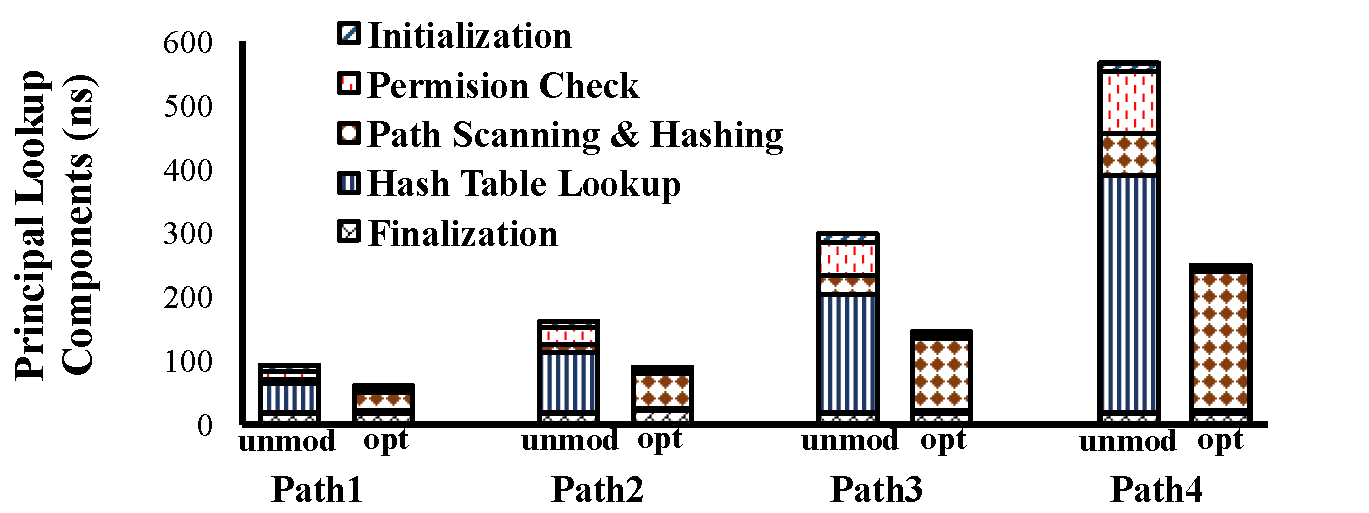
\includegraphics[width=3.6in]{dcache/plots/lookup-breakdown.pdf} \\
\footnotesize
\begin{tabular}{lll}
{\bf Path1:} \tt FFF &
{\bf Path2:} \tt XXX/FFF &
{\bf Path3:} \tt XXX/YYY/ZZZ/FFF \\
\multicolumn{3}{l}{{\bf Path4:} \tt XXX/YYY/ZZZ/AAA/BBB/CCC/DDD/FFF} \\
\end{tabular}
\caption[Principal sources of path lookup latency.]
{Principal sources of path lookup latency in the Linux \linuxver{} kernel. Lower is better.}
%The experiment shows that the latencies of ``Hash Table Lookup'', ``Permission Check'' and ``Path Scanning \& Hashing'' are linear to the number of path components ($O(n)$).
%In our solution, The latencies of ``Hash Table Lookup'' and ``Permission Check'' are constant. }
%\fixmetsai{Maybe we break down the fast path, too?}  } 
%% dp: The fast path would be interesting.  It is a little early here, but let's try it.
\label{fig:dcache:breakdown}
%\vspace{-15pt}
\end{figure}

\subsection{Opportunities for Improvement}

Figure~\ref{fig:dcache:breakdown} shows the time spent in the principal components
of a path lookup in Linux, for four paths of increasing lengths.
The first-order impact on lookup time is the length of the path itself,
which dictates how many times each component will be hashed, looked-up in the 
hash table, and execute a permission check on each directory's inode.
These costs are linear in the number of path components.


The hit latency optimizations described in this paper make most of these 
operations constant time, except for hashing, which is still a function of the 
length of the path.  

%\fixmedp{Here's a radical suggestion: Put the breakdown chart and analysis of opportunities here, not in eval.  It could be a couple
%of stacked bar graphs and a short analysis.}

